
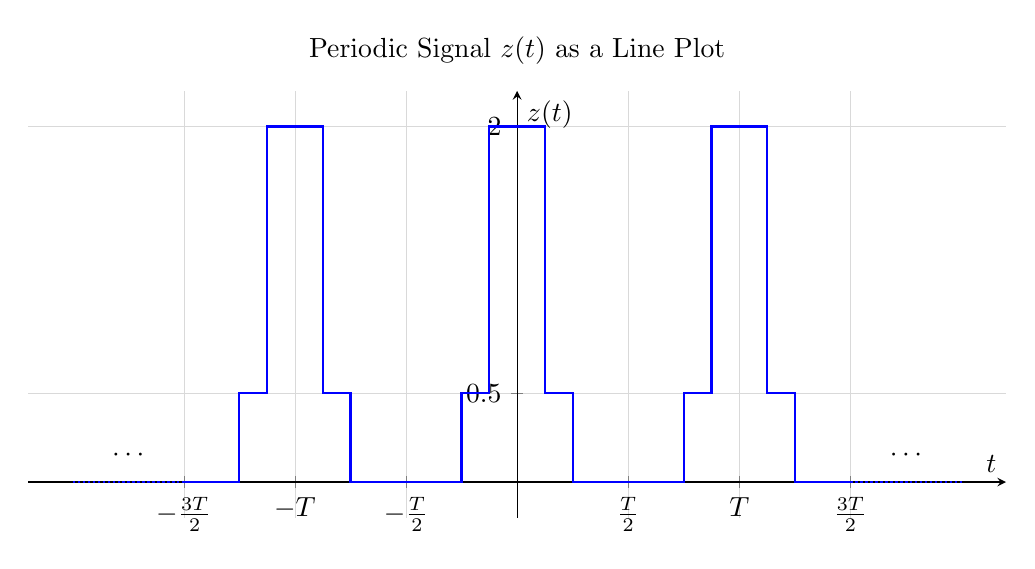
\begin{tikzpicture}
	\begin{axis}[
		% Set the overall style
		width=14cm,
		height=7cm,
		title={Periodic Signal $z(t)$ as a Line Plot},
		xlabel={$t$},
		ylabel={$z(t)$},
		% Position axes at the origin
		axis lines=middle,
		% Set axis limits
		xmin=-2.2, xmax=2.2,
		ymin=-0.2, ymax=2.2, % Lowered ymin slightly for better axis visibility
		% Set symbolic ticks for the period T=1
		xtick={-1.5, -1, -0.5, 0.5, 1, 1.5},
		xticklabels={$-\frac{3T}{2}$, $-T$, $-\frac{T}{2}$, $\frac{T}{2}$, $T$, $\frac{3T}{2}$},
		ytick={0.5, 2},
		% Add a grid
		grid=major,
		grid style={line width=.1pt, draw=gray!30},
		no marks,
		]
		
		% --- Plot each cycle as a single, continuous outline ---
		
		% Cycle 1 (Centered at t = -1)
		\addplot[blue, thick] coordinates {
			(-1.5,0) (-1.25,0) (-1.25,0.5) (-1.125,0.5) (-1.125,2) 
			(-0.875,2) (-0.875,0.5) (-0.75,0.5) (-0.75,0) (-0.5,0)
		};
		
		% Cycle 2 (Centered at t = 0)
		\addplot[blue, thick] coordinates {
			(-0.5,0) (-0.25,0) (-0.25,0.5) (-0.125,0.5) (-0.125,2) 
			(0.125,2) (0.125,0.5) (0.25,0.5) (0.25,0) (0.5,0)
		};
		
		% Cycle 3 (Centered at t = 1)
		\addplot[blue, thick] coordinates {
			(0.5,0) (0.75,0) (0.75,0.5) (0.875,0.5) (0.875,2) 
			(1.125,2) (1.125,0.5) (1.25,0.5) (1.25,0) (1.5,0)
		};
		
		% --- Indicate that the pattern continues ---
		\draw[blue, thick, densely dotted] (axis cs:1.5, 0) -- (axis cs:2, 0);
		\node at (axis cs:1.75, 0.15) {$\cdots$};
		\draw[blue, thick, densely dotted] (axis cs:-2, 0) -- (axis cs:-1.5, 0);
		\node at (axis cs:-1.75, 0.15) {$\cdots$};
		
		% Add period label for one period
		\draw[<->, thick] (axis cs:-0.5, -0.3) -- (axis cs:0.5, -0.3) node[midway, below=2pt] {Period $T = 1$};
		
	\end{axis}
\end{tikzpicture}